\documentclass[journal]{vgtc}                % final (journal style)
%\documentclass[review,journal]{vgtc}         % review (journal style)
%\documentclass[widereview]{vgtc}             % wide-spaced review
%\documentclass[preprint,journal]{vgtc}       % preprint (journal style)

% Colors
\usepackage[
hyperref,% for working together with hyperref
table% for coloring matrix entries
]{xcolor}% color package; load before tocstyle

%% Uncomment one of the lines above depending on where your paper is
%% in the conference process. ``review'' and ``widereview'' are for review
%% submission, ``preprint'' is for pre-publication, and the final version
%% doesn't use a specific qualifier.

%% Please use one of the ``review'' options in combination with the
%% assigned online id (see below) ONLY if your paper uses a double blind
%% review process. Some conferences, like IEEE Vis and InfoVis, have NOT
%% in the past.

%% Please note that the use of figures other than the optional teaser is not permitted on the first page
%% of the journal version.  Figures should begin on the second page and be
%% in CMYK or Grey scale format, otherwise, colour shifting may occur
%% during the printing process.  Papers submitted with figures other than the optional teaser on the
%% first page will be refused. Also, the teaser figure should only have the
%% width of the abstract as the template enforces it.

%% These few lines make a distinction between latex and pdflatex calls and they
%% bring in essential packages for graphics and font handling.
%% Note that due to the \DeclareGraphicsExtensions{} call it is no longer necessary
%% to provide the the path and extension of a graphics file:
%% 
\includegraphics{diamondrule} is completely sufficient.
%%
\ifpdf%                                % if we use pdflatex
  \pdfoutput=1\relax                   % create PDFs from pdfLaTeX
  \pdfcompresslevel=9                  % PDF Compression
  \pdfoptionpdfminorversion=7          % create PDF 1.7
  \ExecuteOptions{pdftex}
  \usepackage{graphicx}                % allow us to embed graphics files
  \DeclareGraphicsExtensions{.pdf,.png,.jpg,.jpeg} % for pdflatex we expect .pdf, .png, or .jpg files
\else%                                 % else we use pure latex
  \ExecuteOptions{dvips}
  \usepackage{graphicx}                % allow us to embed graphics files
  \DeclareGraphicsExtensions{.eps}     % for pure latex we expect eps files
\fi%

%% it is recomended to use ``\autoref{sec:bla}'' instead of ``Fig.~\ref{sec:bla}''
\graphicspath{{figures/}{pictures/}{images/}{./}} % where to search for the images

\usepackage{microtype}                 % use micro-typography (slightly more compact, better to read)
\PassOptionsToPackage{warn}{textcomp}  % to address font issues with \textrightarrow
\usepackage{textcomp}                  % use better special symbols
\usepackage{mathptmx}                  % use matching math font
\usepackage{times}                     % we use Times as the main font
\renewcommand*\ttdefault{txtt}         % a nicer typewriter font
\usepackage{cite}                      % needed to automatically sort the references
\usepackage{tabu}                      % only used for the table example
\usepackage{booktabs}                  % only used for the table example
%% We encourage the use of mathptmx for consistent usage of times font
%% throughout the proceedings. However, if you encounter conflicts
%% with other math-related packages, you may want to disable it.

%% In preprint mode you may define your own headline.
%\preprinttext{To appear in IEEE Transactions on Visualization and Computer Graphics.}

%% If you are submitting a paper to a conference for review with a double
%% blind reviewing process, please replace the value ``0'' below with your
%% OnlineID. Otherwise, you may safely leave it at ``0''.
\onlineid{0}

%% declare the category of your paper, only shown in review mode
\vgtccategory{Research}
%% please declare the paper type of your paper to help reviewers, only shown in review mode
%% choices:
%% * algorithm/technique
%% * application/design study
%% * evaluation
%% * system
%% * theory/model
\vgtcpapertype{VAST}

\title{Interactive Filter and Display of Hillary Clinton's Emails: \\A Cautionary Tale of Metadata}

\author{Christopher D. Salahub and R. Wayne Oldford}
\authorfooter{
%% insert punctuation at end of each item
\item
 Christopher D. Salahub, University of Waterloo, Canada \\E-mail: csalahub@uwaterloo.ca.
\item
 R. Wayne Oldford, University of Waterloo, Canada \\ E-mail: rwoldford@uwaterloo.ca.
}

%other entries to be set up for journal
\shortauthortitle{Salahub and Oldford: Filter and Display of Clinton's Emails}
%\shortauthortitle{Firstauthor \MakeLowercase{\textit{et al.}}: Paper Title}

\abstract{We present a web-based visualization that allows the user to interactively filter and display characteristics of 32,795 Hillary Clinton's emails as provided by Wikileaks.

The visualization focuses on the meta-data of each email, including its senders, receivers, and the timestamp the email appeared on the Clinton server.  An interactive time range slider filters all email and all displays automatically update to changes in the slider.  The main display shows Clinton's most frequent correspondents arranged as nodes of a spoked graph with Clinton at the centre.  Volume determines the thickness of each spoke and high volume determines an inner circle whose spokes are shortened.  Correspondents and their edges are coloured according to whether that email account could be identified as being an approved Federal government account or not.  A second display shows two daily time series: the total number of emails for that day, and the number meeting selection criteria.  A third display shows a scatterplot of the time of day versus the day on which that email appeared.  Scatterplot points are coloured by whether the email was redacted or not.  

Other displays add some information beyond metadata.  FOIA exemption codes appear as a selectable list and a barplot shows email counts by FOIA code.  The (stemmed) terms having highest frequency in the displayed email, and those having highest tf-idf are listed in separate displays.  All displays are interactively filtered by time range and selected FOIA codes.

We illustrate how the filtered displays can be used to generate hypotheses and uncover interesting information.  These touch on contentious issues including the handling of classified information, the 2012 attack on the Benghazi U.S. diplomatic compound, and emails apparently missing from those released publicly.  

The data are extracted from Wikileaks HTML files, cleaned, and stored in a form useful for interactive exploration.  A local \texttt{R} \texttt{shiny} server provides the interactive displays as a public service online tool to explore and uncover patterns in the meta-data and summary contents of Clinton's email.  Coupled with publicly available sources of information, these interactive tools uncover surprising amounts of information about an individual, especially one holding public office. The ease with which this can be accomplished and shared should serve as a clear warning as to what can be learned about anyone from metadata.
}

%% Keywords that describe your work. Will show as 'Index Terms' in journal
%% please capitalize first letter and insert punctuation after last keyword
\keywords{Exploratory data analysis, metadata, text mining, web-scraping, interactive web visualization,  \texttt{R},  \texttt{shiny} }

%% ACM Computing Classification System (CCS). 
%% See <http://www.acm.org/class/1998/> for details.
%% The ``\CCScat'' command takes four arguments.

\CCScatlist{ % not used in journal version
 \CCScat{K.6.1}{Management of Computing and Information Systems}%
{Project and People Management}{Life Cycle};
 \CCScat{K.7.m}{The Computing Profession}{Miscellaneous}{Ethics}
}

%% Uncomment below to include a teaser figure.
\teaser{
  \centering
  \begin{tabular}{cc}
  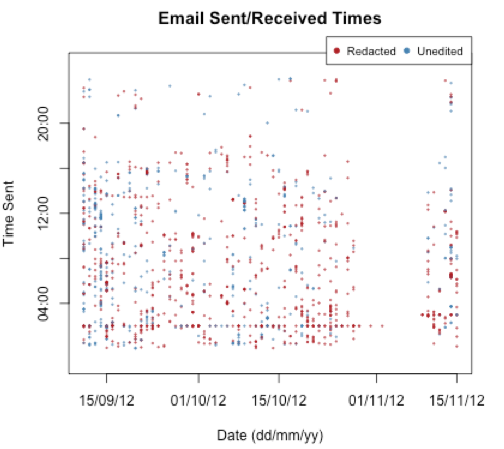
\includegraphics[width=0.25\textheight]{DailySept11ToNov152012_All} &
  \includegraphics[width=0.25\textheight]{InnerCircleSept11ToNov152012_All} \\
  &\\
  {\small (a) Missing data in November.} & {\small (b) Inner Circle: Correspondent info by colour; volume by thickness.}
  \end{tabular}
  \caption{Metadata: Time, date, correspondents, volume.  Filtered: Sept. 11 to Nov. 15, 2012.  
  %Source: \href{https://wikileaks.org/clinton-emails/}{\texttt{https://wikileaks.org/clinton-emails/}}
  }
  
	\label{fig:teaser}
}

%% Uncomment below to disable the manuscript note
%\renewcommand{\manuscriptnotetxt}{}

%% Copyright space is enabled by default as required by guidelines.
%% It is disabled by the 'review' option or via the following command:
% \nocopyrightspace

\vgtcinsertpkg

%%%%%%%%%%%%%%%%%%%%%%%%%%%%%%%%%%%%%%%%%%%%%%%%%%%%%%%%%%%%%%%%
%%%%%%%%%%%%%%%%%%%%%% START OF THE PAPER %%%%%%%%%%%%%%%%%%%%%%
%%%%%%%%%%%%%%%%%%%%%%%%%%%%%%%%%%%%%%%%%%%%%%%%%%%%%%%%%%%%%%%%%

% Commands with arguments
\newcommand*{\TODO}[1]{\textcolor{red}{TODO #1}}
% See http://tex.stackexchange.com/questions/251460/how-to-put-symbols-of-equal-size-on-top-of-each-other?noredirect=1#comment599930_251460

\begin{document}
%% the only exception to this rule is the \firstsection command
\firstsection{Introduction}
\maketitle
The 2016 U.S. Presidential election was one of the most contentious in history.  The existence and possible content of Hillary Clinton's private email server dogged former Secretary Clinton's bid for the U.S. presidency and was doubtless a contributing factor to her surprising defeat by Donald Trump.

On March 16, 2016 Wikileaks  published a searchable archive \cite{Wikileaks} containing the contents of more than 30,000 emails (and attachments) that were sent to and from Secretary Clinton's private server.  The documents were provided as pdfs by the U.S. Department of State in response to Freedom of Information Act (FOIA) \cite{FOIA} requests.  The State Dept. also provided a searchable web archive of the pdf documents, released in several installments from May 2015 to March 2017\cite{StateDeptFOIA}.   Both sites provide a  useful tool for anyone searching for particular terms in the documents.  The Wikileaks site was put to much use by investigative reporters, and others, to search for topical news items.

What is critically missing from either site, however, is the ability to easily conduct statistical analyses of their contents.  Only then can patterns be easily discerned.  

In this paper, we describe a complementary website service (\texttt{rshiny.math.uwaterloo.ca/clinton}).  This service does not provide the search facilities found on Wikileaks, but rather provides the user with interactive visualizations that allow them to uncover patterns in the emails and, through a variety of filters on the emails,  to explore these patterns at some depth.  The service is intended to be used in conjunction with either the Wikileaks service or the State Dept. FOIA service.   The latter two provide the search mechanisms as well as the actual contents of individual emails.  One imagines having three browsers open, one for the data base search (e.g. Wikileaks), one for statistical visualization and exploration (our service), and one for internet search (to provide important context for the other two services). Each one fills a need not met by the other two; the synergy of all three provide the user a powerful set of investigative tools.

In providing the service, we have purposely restrict consideration (for the most part) to displaying patterns of simple characteristics of the emails, the so-called metadata. The reasons for this are two-fold. The first is that for this data the metadata is simply more reliable and regular. The emails are often heavily redacted, and this introduces both gaps in content and irregularities. The metadata, however, remains somewhat informative and regular in format despite redactions, as the only redacted metadata is that of individual email addresses, and noting these redactions is in itself useful. The second reason is demonstrate the power of supported metadata in the exploration of communication data. For public figures in particular, a communication network plot and time-stamps can be very easily leveraged for insightful data exploration if outside sources are consulted. The individual's communication habits can be extended to gain insight into their general habits in life, while the individuals they communicate with most frequently can establish interesting connections which might otherwise be missed, such as that between Clinton and Tony Blair.


\TODO{MORE TO COME HERE}

Meta data ...  Cautionary

\subsection{A brief timeline on the private email server}
While the following timeline is somewhat abbreviated, it should serve to raise some of the major issues and concerns related to the private email server and its contents.  It also introduces some of the principal characters in the whole affair.  More complete and in depth timelines are readily available on the internet (e.g. \cite{attkissonTimeline, thompsonTimeline, WashPostTimeline, clintonWikipedia, TimeMagEverything}).

On November 21, 2008, the New York Times reported that Hillary Clinton had decided to accept the position of U.S. Secretary of State.  On January 13, 2009 the internet domain name \texttt{clintonemail.com} was registered \cite{whoisClintonserver}; eight days later Senator Clinton was confirmed as Secretary of State.  

Public knowledge that a private email server being used by Secretary Clinton and others for State Department and personal communications did not surface until March 2015 \cite{NewYorkTimes2015} during the course of a U.S. Congressional investigation \cite{BenghaziReport} of the September 11, 2012 attack by militants on U.S. compounds in Benghazi Libya.  

The State Department had difficulty fulfilling public FOIA and House Benghazi Committee requests \cite{TakingRootWashPost} for Secretary Clinton's government emails because she had exclusively used the private server for all her email.  On March 10, 2015,  Clinton told reporters that she turned over 30,490 emails to the State Department and deleted 31,830 emails deemed to be personal \cite{WashPostTimeline}.    Clinton had tasked three lawyers Cheryl Mills (Clinton's former chief of staff),  David Kendall (Clinton's personal lawyer), and Heather Samuelson (a State Department staffer during Clinton's tenure) to make the determinations as to which emails were work related and which were not \cite{emailVetting, thompsonTimeline}.   

On March 10, 2015 the House Benghazi Committee requested that the private email server be turned over to a neutral third party to determine which emails are personal and which are government records \cite{serverRequest}, but was informed March 27 by David Kendall that no emails remained on the private server for any kind of review \cite{serverScrubbedLawyer}.
Between March 25 and 31, 2015, Paul Combetta (then the server's system administrator), erased all backup copies using \texttt{BleachBit} (see \texttt{www.bleachbit.org}).    

Combetta, Mills, and Samuelson will later be granted partial immunity by the Justice Department during the FBI investigations into the private email server, as were two others: Bryan Pagliano (original server manager) and  John Bentel (former director of Information Resources Management for the State Department's Executive Secretariat) \cite{immunityPolitico, immunityDailyCaller, immunityIT}.  

On April 12, 2015 Clinton announces that she is running for the U.S. Presidency.  On July 24, 2015, inspectors general for the State Department  and the national intelligence agencies announce finding classified information in the emails and that the information they found was classified at the time sent \cite{serverClassified}, though her campaign declared that they must have been classified after the fact. On August 19, 2015, Clinton calls the allegation of mishandling classified information a ``disagreement between agencies'' \cite{clintonDenialGuardian}.

Nearly one year later, July 5, 2016,  FBI Director James Comey recommended that no charges be laid against Clinton on use of private email server \cite{nochargeFBI}.  On October 28, 2016, Comey revealed that in a separate investigation into former Congressman Anthony Weiner, that emails belonging to his wife Huma Abedin have been found on his laptop.  Since Abedin was a close aid to former Secretary Clinton, FBI investigations were reopened into the private server usage but closed again by Comey on November 6, 2016 without charges being laid \cite{nochargeFBINov}.  In both cases, Comey and the FBI are criticized by pundits from different political parties.

\section{Old stuff}
\TODO{This material is to be reused wherever}
All work related emails were eventually released to the State Department who subsequently published more than 30,000 on the U.S.  To add to the confusion, only those work government emails, as vetted Secretary Clinton's lawyers 

The emails and the server became a source for criticism of Secretary Clinton, and others, and came to dog her bid for the presidency in 2016, in what may be one of the most contentious U.S. elections in history.   Part of this criticism was levelled  More complete timelines are publicly available on the internet (e.g. \cite{attkissonTimeline, TimeMagEverything, clintonWikipedia}).  For our purposes, it is enoug
 
 
 33,000 supposedly missing emails
 Encouraged 
 and three other American citizens.  Public knowledge of the private email server surfaces State business being conducted on a private server surfaced only after the a

The 2016 US Presidential election was one of the most contentious in history.  The existence and possible content of Hillary Clinton's private email server played a significant role in the campaign until the end.  

The timeline of events related to use of this private server may be found elsewhere (e.g. 
Despite their significant nature, very few of the individuals commenting on the significance of this server had spent any significant time viewing this content. This is no fault of theirs, the officially released data has previously only been stored in databases on the United States' State Department Website (see https://foia.state.gov/Learn/New.aspx) and Wikileaks (see https://wikileaks.org/clinton-emails/) in individually searchable form. Furthermore, the email data is stored in the inconvenient format of individual PDF documents, and in the case of Wikileaks a slightly more convenient but still cumbersome HTML representation based on the official PDF content. This granularity and separation of individual emails on different webpages prevents a great deal interesting analysis of the data, including any aggregate analyses of patterns in content or metadata. As such, the emails are incredibly misunderstood documents, and current searches for patterns and points of interest have relied upon searching for terms of interest and sifting through the results of the search. Such a method is not only tedious but problematic from a statistical point of view, as approaching any data set with a specific hypothesis before exploring its structure and patterns in abstract leads to biased conclusions and poor analysis. In the interest of simplifying the general exploration of this important data set, the Wikileaks HTML email versions were extracted and a series of visualizations were generated around the metadata included in these emails. An interactive web application in \texttt{R} \texttt{shiny} was constructed utilizing these visualizations and the extracted data. Incorporated in this app was a short article explaining the use of the app, providing links to background information, and outlining some of the findings of the more interesting trends observed. This framework provides any individual with interest the ability to generate hypotheses by exploring the data without necessarily searching for any particular conclusion. 

In generating and exploring this data, a considerable amount of respect is gained for the power of the often overlooked metadata of emails, especially with public figures. Simply having access to the network of communications, simple indicators of identifiable features of the individuals communicating, and times sent is enough to generate interesting questions which simple Google searches of important events and days can shed a great deal of light on. Leveraging data beyond this metadata, including the Freedom of Information Act (FOIA) exemption codes (see https://vault.fbi.gov/explanation-of-exemptions) used to redact the emails, only bolsters this simple metadata driven investigation. Metadata is often viewed as less significant or somehow less intrusive data, but the exploration performed in this paper demonstrated, at the very least to the authors, what a powerful tool metadata is for generating hypotheses about data. Given the lack of privacy present in the modern internet age and the amount of information most individuals make publicly available, there is a clear warning here about the utility of metadata for bad or for good. For a public official like Hillary Clinton, the data become even more interesting due to a number of contentious issues which arose during her tenure as the Secretary of State, independent of and as a result of her use of a private server.

\section{Data}

\TODO{This needs to be short and to the point.  Just say what is done.}
HTML versions of the emails were pulled programmatically from the Wikileaks database, as the storage structure supported programmatic extraction using web-scraping and string parsing tools in \texttt{R}. In particular, the packages \texttt{RCurl} and \texttt{XML} proved invaluable to extract the raw HTML pages for each email, and the packages \texttt{tm}, \texttt{stringr}, and \texttt{SnowballC} were indispensible to process and clean the raw HTML into a useable form. After downloading the raw HTML and extracting the data of interest, the resulting data was stored in csv files to provide the flexibility to load the data into any architecture or analysis tool desired.

The PDF files released by the state department used to generate the Wikileaks HTML emails do not include the typical email server header with time stamp information, email addresses, and other regular data. Instead, these files are more similar to screen captures of the emails, providing only the visual display a user would see without the useful information used to generate that display. As a result, the data is very irregular: email addresses are occasionally not included, there were initially concerns over the time zones used to generate the time stamp metadata, and there are doubtless still many fringe cases of irregular spacing or placement of text within the HTML code not considered in cleaning. While the metadata is relatively consistent in spite of these irregularities, there are still impure and messy addresses and contact names arising from these irregularities.

After the emails were pulled, stopwords defined by the \texttt{stopwords} function from \texttt{tm} were removed and the remaining words were stemmed by the \texttt{stemDocument} function from \texttt{tm} and \texttt{SnowballC}. Both of these seemed imperfect and ill-suited to the data, failing to remove words with little informative power and creating often cryptic stems.

\section{Displays}
\TODO{Each of these four displays is described and commented on in context of whole time line}
\subsection{Inner circle} 
The spokes are separated into two groups by the radial length of the spokes, these groups are determined automatically by the largest difference in volume of correspondence present in the data between the ordered counts of number of emails sent between individuals. As well, the width of the edges of the graph is determined by the volume of correspondence which occurred between Clinton and the correspondent in either direction. Finally, all edges and points are coloured according to a simple scheme: if the name associated with a node in the graph is at any point associated with an email address hosted at some '.gov' domain in the correspondences, their node is coloured blue; nodes with email addresses which are identifiably not hosted at a '.gov' domain are coloured red; nodes with '.mil' accounts are coloured black; and nodes unidentifiable hosts are coloured orange. It is important to note that for those individuals with orange spokes, the most likely reason the email is not identifiable is the redaction of the email by the state department. Such a redaction is not a guarantee that the email of the individual is not an official state email, but it is an indication that the email address is viewed as personal or private information, which suggests some email hosted outside of the '.gov' domain.

\subsection{Email volume}
This plot has two lines, the first is a line showing the total volume of emails for each day, and the second shows the number of emails satisfying the classification filter criteria for a given day. This allows users to view which days have an exceptionally high or low number of classified conversations. Returning to the motivation of hypothesis generation, referencing world events on any days of interest provides a number of interesting insights on how public figures like Clinton react and respond to world events.

\subsection{Email times}
This plot takes advantage of the time-stamps on every email and then plots the emails as points with times on the vertical axis and the day sent on the horizontal axis. The points in this scatterplot are then coloured according to whether the corresponding email was redacted, in which case the point is coloured red, or released in full, in which case the point is coloured blue. Alpha blending and transparency of these points was utilized to make the patterns present more obvious and prevent overplotting from obscuring any interesting results. 

One such result which is immediately obvious is the strange pattern of sending times. Email communications occur with the highest frequency between midnight and 3 am, and with the lowest frequency between 4 pm and 10 pm. This pattern, which is persistent through filters of emails sent to Clinton and by Clinton, is surprising as it indicates that the highest level of communication was occurring at a time typically devoted to sleep. Another pattern immediately obvious is the alternating modes at 2 and 3 am, with alternations occurring on the dates of daylight savings in North America. The regularity of this pattern in the emails suggests some server function performed early in the morning, perhaps some maintenance operation performed every 24 hours.

\subsection{FOIA exemptions}.
 The United States Freedom of Information Act (FOIA) exemption codes \cite{FOIA} are used by the United States Federal Government to remove sensitive information from released documents accessed using a Freedom of Information Act request. The sensitive matters being addressed by the codes are national security and foreign policy matters for B1, personnel practices for B2, exempted by statute for B3, trade secrets or financial information obtained in confidence for B4, inter- or intra-agency memorandums for B5, personal privacy for B6, records compiled for law enforcement for B7, prepared in relation to financial monitoring institutions for B8, and geophysical and geological information concerning wells for B9 exemptions. The frequencies of each of these codes within filtered emails are shown in the final display. Note that as emails can have numerous redaction codes, this barplot can be useful to identify which codes co-occur over a selection.

\subsection{Term frequency and TFIDF}
The term frequency and tf-idf displays for this data are perhaps the least directly useful. As mentioned above, the stemming and stopword removal provided by the package \texttt{tm} in \texttt{R} proved inadequate for the messy and non-standard data. In particular, the omission of many common and uninformative action verbs such as 'will' and 'can' from the stopwords used led to very unsatisfactory results. A set of custom stopwords was therefore applied in an attempt to remove some of these uninformative words. The tf-idf was more informative, but the stemming algorithm, when coupled with the typos and abbreviations which are incredibly common in the emails, meant that the results are still incredibly unclear. The terms with the highest scores over any interval do not seem to communicate anything particularly useful about the content of emails sent in that range, with one notable exception in the case of the term 'windrush.' This term appeared with a high tf-idf in a number of selections which contained communications with Tony Blair (email contact "aclb" in the spiral plot), and seems to refer to Windrush Ventures, a company owned by Blair which appears vital in managing Blair's complicated and opaque finances since he left the office of the Prime Minister of the United Kingdom. \cite{windrushTelegraph, windrushGuardian}

\section{Filters}
\TODO{Each filter is described and displayed }
\subsection{Time filtering}
Time filtering within the app can be completed at the level of individual days. The use of the mouse to click and drag the slider boundaries allows for large, rapid changes in the date range specified, while clicking on one of the boundaries and using the arrow keys allows for fine selection of the date range via single days. As well, clicking and dragging the blue bar in between the boundaries allows the user to sweep the data with an interval of a fixed width. Clicking the middle bar and using the arrow keys allows the user to shift the range selected by individual days, analogously to the boundaries.
\subsection{Sent or received}
A drop down menu allows users to select emails by those sent to Clinton, sent by Clinton, or by the entire email database.
\subsection{FOIA exemptions}
Multiple filtering by FOIA exemption codes is supported in the app with a box selection area. Users can add FOIA exemption codes currently not included to the data by clicking the box with their mouse and selecting a code from the menu which is then displayed below the box. To remove codes, the user simply clicks the code within the display box and presses delete, which moves the code to the selection menu. The box therefore displays all codes currently included in the data displayed.
\subsection{Auxiliary information}
\TODO{e.g. Clinton's foreign schedule}
A number of cosmetic adjustments using auxiliary information can also be made. Users can choose to adjust the scatterplot of time by day, which re-defines 6 pm as the time at which the day changes. This simply groups the emails best, placing all emails into one mostly uninterrupted region by redefining the day about the midsection of the region of lowest email traffic. Another cosmetic adjustment is the inclusion of Clinton's foreign trip schedule as blue regions on the email volume plot. This schedule was taken from the official State Department website \cite{ForeignSched} and allows users to distinguish periods spent out of the United States (coloured in blue) from those spent within the United States (uncoloured).
\section{Some further exploration}
\TODO{Some of our findings.  Unless done in the previous section}
\section{Shiny App}
\TODO{Again short and to the point}
The \texttt{R} \texttt{shiny} app at (HOST ADDRESS) provides the ability for users to interactively filter the data on all features described above and view the resulting displays. Alongside this display is a short article explaining the use of the app, providing links to background information, and outlining some of the more interesting trends observed. It is hosted on the Waterloo \texttt{rshiny} server for public access, allowing for any individual to make use of this tool to generate hypotheses and investigate this intriguing dataset.


Historically important,  possibly had an impact on the 2016 US presidential election.

Contentious issues:
\begin{itemize}
\item private email server
\item classified documents (outside of state)
\item Sidney Blumenthal
\item Benghazi spin handling of media (Susan Rice)

\item scrubbing of her server (bleachbit)
\item missing email from online email State department
\end{itemize}


Learn:
\begin{itemize}
\item inner circle over time (state or not)
\item spike in email around Libyan revolution
\item gap in the email
\item daily email patterns, server behaviour (daylight savings time)
\end{itemize}

  
 Filter:
\begin{itemize}
\item time
\item redacted or not
\item FOIA exemption codes
\end{itemize}

   
 Content:
\begin{itemize}
\item Term frequency, TFIDF
\end{itemize}

   
 Tool: 
\begin{itemize}
\item Web-based, interactive filter and display tool
\end{itemize}
    
    
Discovery from visualization \& connecting discovery sources



- Nothing on this ... Preparation for Benghazi (security considerations)

- House Oversight and Government Reform Committee (standing committee) 
  Darrell Issa, Chair
     Jason Chaffetz, Chair (Gowdy a member)
  (discovered email server)
    ... 
- House Select Committee on Benghazi (Summer 2014) 
   Trey Gowdy, Chair

\section{Exposition}


%% if specified like this the section will be committed in review mode
\acknowledgments{
This work was supported in part by
a Discovery grant from the Natural Sciences and Engineering Research Council of Canada..}

\newpage
\bibliographystyle{abbrv}
%\bibliographystyle{abbrv-doi}
%\bibliographystyle{abbrv-doi-narrow}
%\bibliographystyle{abbrv-doi-hyperref}
%\bibliographystyle{abbrv-doi-hyperref-narrow}

\bibliography{clinton}

\end{document}
